\documentclass[sigconf,nonacm]{acmart}
\settopmatter{printacmref=false}
\renewcommand\footnotetextcopyrightpermission[1]{}
\pagestyle{plain}
\usepackage{amsmath}
\newcommand{\fillin}[1]{\textcolor{red}{[#1]}}
% #RUNNING-TODO: every \runningtodo{...} marks a number that depends on a run still in progress.
% Search this file for "#RUNNING-TODO" to find them all.
\newcommand{\runningtodo}[1]{\textcolor{orange}{\textbf{\#RUNNING-TODO}: #1}}

\begin{document}

\title{AgentIR Milestone Report}
\subtitle{Agentic Image Retrieval --- CS5787 Deep Learning, Cornell Tech, Fall 2026}

\author{Usman Ali}
\affiliation{\institution{Cornell Tech}\city{New York}\country{USA}}
\email{ua49@cornell.edu}

\author{Nophar Shalom}
\affiliation{\institution{Cornell Tech}\city{New York}\country{USA}}
\email{ns2242@cornell.edu}

\author{Kenechukwu Okoroafor}
\affiliation{\institution{Cornell Tech}\city{New York}\country{USA}}
\email{kao92@cornell.edu}

\renewcommand{\shortauthors}{Ali, Shalom and Okoroafor}

\begin{abstract}
Chat-based image retrieval systems such as ChatIR and PlugIR find a target image in a large
corpus by asking the user questions and rewriting the search query after each answer. We are
building an agent that can also issue its own probing searches between questions. For the
milestone we reproduced the PlugIR baseline inside a modular framework, \textsc{AgentIR}, checked
where the baseline loses the target, and re-ran seven variants end to end on the same 200 randomly
sampled VisDial dialogs with an open model (Qwen3.5-9B). Vanilla PlugIR reaches 93.5\% Hits@10
after ten rounds. No variant so far moves this by more than two points, including an upper bound
that always shows the questioner the target's caption, while several changes that looked large in
offline analysis disappear end to end.
\end{abstract}

\maketitle

%====================================================================
\section{Introduction and background}
Text-to-image retrieval ranks the images of a corpus by how well they match a textual
description. A single caption is often ambiguous: in the ChatIR example the target starts at
rank 1{,}149 among 50K images~\cite{levy2023chatir}. \emph{ChatIR}~\cite{levy2023chatir} turns
retrieval into a dialog: an LLM asks questions, a simulated user answers them from the target
image, and the growing dialog is used as the query. \emph{PlugIR}~\cite{lee2024plugir} conditions
each question on the images the current query retrieves: it clusters the retrieved candidates,
shows the questioner one caption per cluster, filters questions the candidates already answer,
picks one by a KL criterion, and rewrites the dialog into a single caption-like query before each
search. PlugIR also introduced the Best log Rank Integral (BRI) metric.

Both systems pay for accuracy with user effort: every round needs the user to read and answer a
question. Our project, proposed by our advisor Matan Levy, gives the agent its own search actions,
so it can probe the corpus between questions, both to ask more discriminative questions and to find
the target with fewer rounds. \textbf{Research question:} \emph{can an agent that issues its own
searches find the target faster, or with fewer user answers, than PlugIR?} Before adding probes we
needed a faithful, instrumented PlugIR baseline and an understanding of where the current loop
loses the target. That is the scope of this milestone.

%====================================================================
\section{Related work}
\textbf{A2R} (Ask-to-Retrieve)~\cite{a2r} is the closest follow-on work. Instead of PlugIR's
cluster captions it shows the questioner a grid of candidates selected from the top 50 to be both
relevant and diverse with a determinantal point process (DPP)~\cite{kulesza2012dpp}, and it scores
candidate questions by their expected information gain over those candidates, estimated with a VQA
model. We use A2R's DPP selector as one of our evidence baselines and its information-gain
scoring in our question-transfer analysis.
Information-gain question selection for grounded retrieval goes back further; Keh et
al.~\cite{keh2024asking} show that VQA presupposition errors break naive information gain and
filter irrelevant images before scoring open-ended questions. \textbf{DAR}~\cite{long2025dar}
keeps the dialog loop but adds diffusion-generated images as intermediate query representations,
improving interactive retrieval without fine-tuning. Our selectors also borrow two classic
retrieval tools: maximal marginal relevance (MMR)~\cite{carbonell1998mmr} for diverse selection
and reciprocal-rank fusion (RRF)~\cite{cormack2009rrf} for combining queries.
None of these methods lets the questioner issue its own exploratory searches, which is the gap our
agent targets.

%====================================================================
\section{Problem and evaluation setup}
\label{sec:formal}
\paragraph{Data.} The corpus $\mathcal{D}$ has $|\mathcal{D}|=50{,}000$ images: the targets of the
2{,}064 VisDial~\cite{das2017visdial} validation dialogs used by PlugIR, plus COCO
\texttt{unlabeled2017}~\cite{lin2014coco} distractors, following the ChatIR/PlugIR protocol. Each
dialog $n$ has a target $I^*_n\in\mathcal{D}$ and an initial caption $c_n$. Images and text are
embedded with frozen BLIP ITM-large encoders~\cite{li2022blip}, $v_j=E_i(I_j)$ and $E_t(\cdot)$;
image embeddings are computed once and cached. No model is trained.

\paragraph{Split.} Offline analyses replay all 2{,}064 released PlugIR dialogs (or a 500-dialog
subset) or 100 saved development states. All new end-to-end runs use the same \textbf{200
dialogs}, drawn uniformly from the 2{,}064 with a fixed seed (20261112), for the full 10 rounds.

\paragraph{Interaction.} At round $r=0$ the query is $q_0=c_n$. In each round $r=1,\dots,R$
($R=10$) the agent asks a question $Q_r$; the user simulator, which sees only $I^*_n$, answers
$A_r$; and the agent produces a new query $q_r=f(c_n,(Q_1,A_1),\dots,(Q_r,A_r))$. The rank of the
target under $q_r$ is
\begin{equation}
\rho_{n,r}=1+\big|\{j:\ \langle E_t(q_r),v_j\rangle>\langle E_t(q_r),v^*_n\rangle\}\big|.
\end{equation}
The agent never observes $I^*_n$ or $\rho_{n,r}$.

\paragraph{Metrics.} Over $N$ dialogs and for every round $r$,
\begin{align}
\text{Hits@}K(r)&=\tfrac{1}{N}\textstyle\sum_n \mathbb{1}\big[\min_{t\le r}\rho_{n,t}\le K\big],\\
\text{Recall@}K(r)&=\tfrac{1}{N}\textstyle\sum_n \mathbb{1}[\rho_{n,r}\le K].
\end{align}
\textbf{Hits@10 is our primary metric}: the user would have seen the target in the top 10 at some
round. Recall@10, which drops if a later rewrite loses the target, is secondary. For comparability
with PlugIR we also report
$\text{BRI}=\frac{1}{N}\sum_n \frac{1}{R}\int_0^R \log\big(1+\min_{t\le r}\rho_{n,t}\big)\,dr$
(trapezoid rule, lower is better). Differences between methods are paired over dialogs, with 95\%
bootstrap intervals.

%====================================================================
\section{Method and implementation}
\label{sec:method}
\subsection{Reproducing the PlugIR baseline}
At round $r$ the questioner's candidate pool is the top $n_r$ images under $q_{r-1}$, with
$n_r=500-50(r-1)$ (500 down to 50). The pool is clustered into $K=10$ groups with spherical
$k$-means. In each cluster, PlugIR shows the caption of the image whose caption-similarity
distribution over the pool,
$p_i=\operatorname{softmax}(\{\langle E_t(\text{cap}_i),v_j\rangle\}_j)$, has the lowest entropy.
An LLM generates $M=5$ questions from these captions and the dialog, drops the ones the captions
already answer, and the ranker keeps
$\arg\min_Q \mathrm{KL}\big(p(\cdot\mid q_{r-1})\,\|\,p(\cdot\mid q_{r-1}\oplus Q)\big)$ over the
images ranked 11 to $n_r$. The reformulator asks the LLM to rewrite the caption and all answers as
one description. We replaced ChatGPT and BLIP-2 with Qwen3.5-9B~\cite{qwen35} as questioner,
rewriter and simulated user (a vision-language model that sees the target image), served 4-bit with
Ollama on one Colab L4 GPU.

\subsection{What is working in the repository}
\textsc{AgentIR} splits the agent into three replaceable modules and runs it against a separate
user-simulator service, in process or over HTTP:
\begin{enumerate}
\item \textbf{Generator}: builds the evidence shown to the questioner and asks the LLM for
  candidate questions, then filters them.
\item \textbf{Ranker}: selects one question.
\item \textbf{Reformulator}: rewrites the dialog into the next query $q_r$.
\end{enumerate}
A \texttt{SearchTool} gives the agent metered access to the retriever, so every probe the agent
issues is counted as a cost per round. Each configuration is a YAML file with a fingerprint, runs
resume after interruptions, and LLM calls are cached. Working today: the PlugIR port, every variant
below, the evaluator (Hits@$K$, Recall@$K$, BRI, bootstrap), diagnostic scripts, plotting, a
Colab notebook that runs the full 200-dialog comparison, and 31 unit tests including metric parity
with PlugIR's \texttt{eval.py}.

\subsection{Variants under test}
Each variant changes one module and keeps the rest of PlugIR fixed. Let $P_r$ be the clustered
pool, $S_r\subset P_r$ the 10 images whose captions are shown, and $\mathrm{top}_k(q)$ the $k$
best-ranked images under $q$.
\begin{itemize}
\item \textbf{Evidence selection (E1, S3).} \emph{Best-ranked representatives}: $S_r$ takes the
  best-ranked image of each cluster instead of the lowest-entropy one. \emph{Fixed pool}:
  $P_r=\mathrm{top}_{500}(q_{r-1})$ or $\mathrm{top}_{100}(q_{r-1})$ for every round.
  \emph{Selectors}: $S_r$ chosen from a 50-image pool by MMR or by fused top-10 ranking, scored
  with the current query or with the whole query history.
\item \textbf{History pooling (S2).} $P_r=\mathrm{top}_{100}\big(\bigcup_{t<r}\mathrm{top}_{200}(q_t)\big)$,
  re-ranked by $q_{r-1}$. Its matched baseline is $P_r=\mathrm{top}_{100}(q_{r-1})$.
\item \textbf{Query fusion (S1).} Rank by RRF of $q_0$ and $q_r$, or prepend $c_n$ to $q_r$.
\item \textbf{Upper bound.} Replace one element of $S_r$ (at a seeded random slot) with the target
  $I^*_n$ every round. This deliberately cheats: it measures how much the loop can gain if the
  evidence always contains the target.
\item \textbf{Agentic ranker (implemented, not yet run at scale).} For each candidate question $Q$
  the LLM proposes 2--3 plausible answers $a_1..a_m$; each answer becomes a hypothetical query
  $q_{r-1}\oplus(Q,a_i)$ that is \emph{issued as a probe}; the question whose answers give the most
  divergent result sets (Jaccard or Jensen--Shannon divergence) is asked. This is the first use of
  the agent's own search actions.
\end{itemize}

%====================================================================
\begin{figure*}[t]
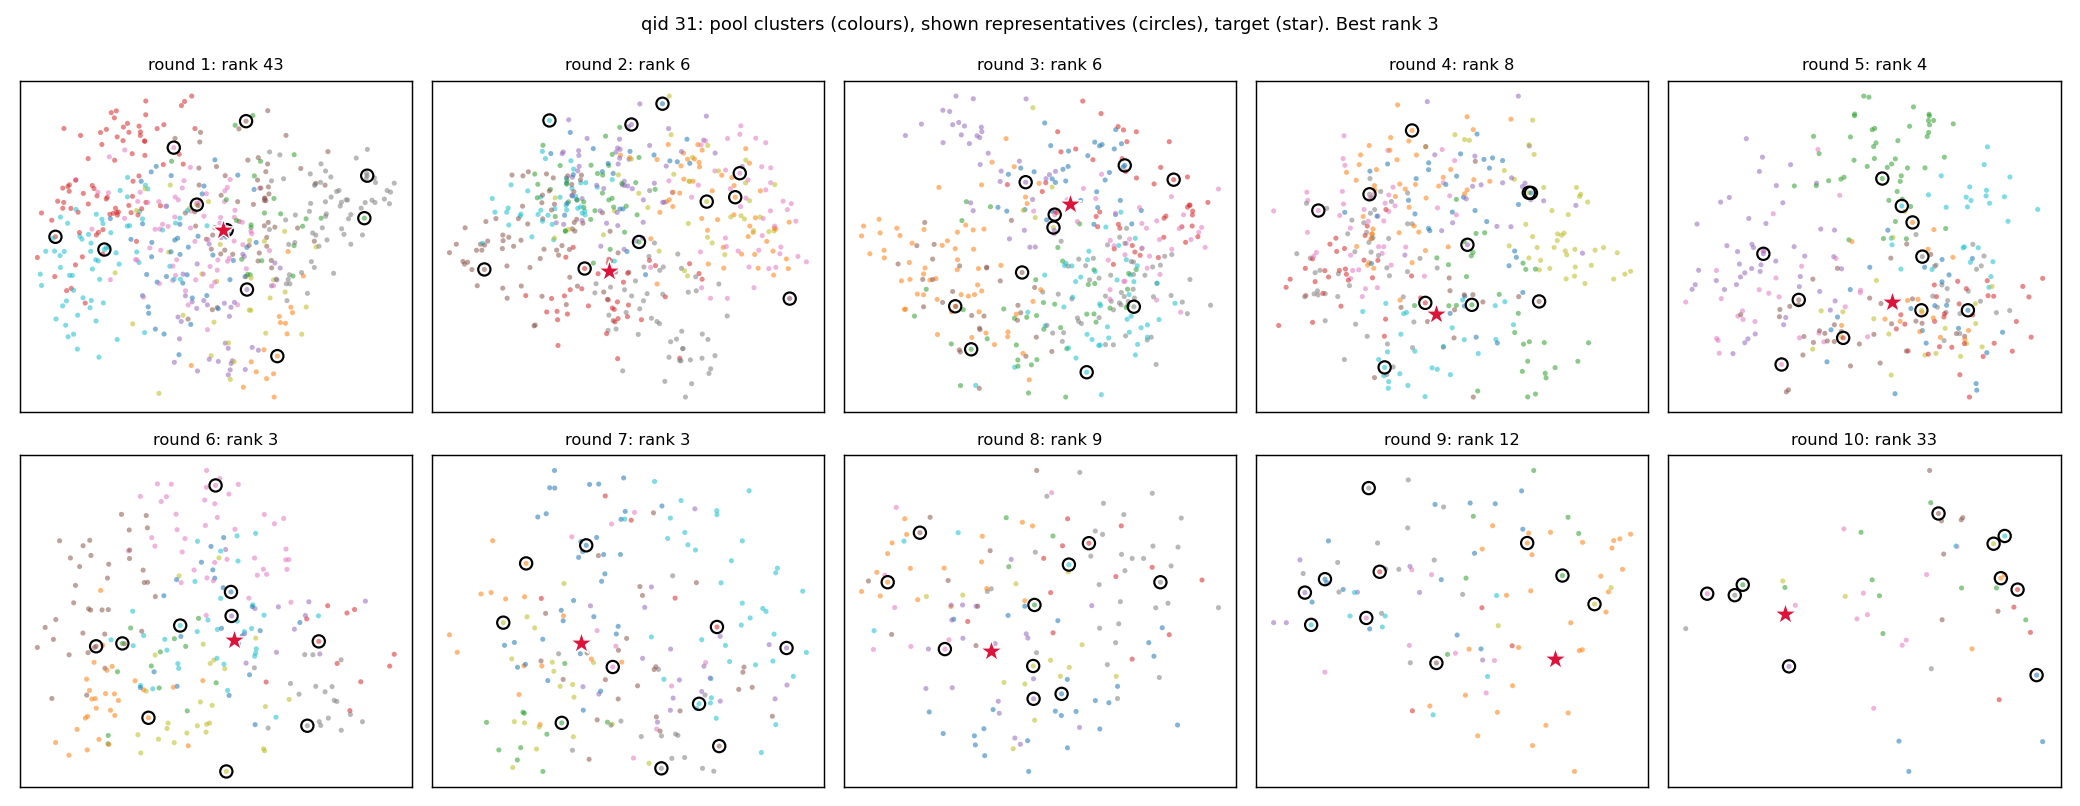
\includegraphics[width=\textwidth]{clusters_qid31.png}
\caption{One vanilla PlugIR dialog, rounds 1--10: the questioner's candidate pool projected to
2-D (colours: $k$-means clusters; circles: the 10 shown representatives; star: the target).
The target reaches rank 3 at round 6 and falls to rank 33 by round 10.}
\label{fig:clusters}
\Description{Ten scatter plots of shrinking image pools with cluster colours and a red star for the target.}
\end{figure*}

\section{Preliminary results}
\subsection{PlugIR baseline checks}
\label{sec:checks}
\paragraph{Baseline result.} On PlugIR's released dialogs our retriever and evaluator give BRI
0.768 against the 0.767 reported by PlugIR, so retrieval and scoring match the paper. With
Qwen3.5-9B in place of ChatGPT, vanilla PlugIR on our 200 dialogs reaches 70.0\% Hits@10 from the
caption alone and 93.5\% after ten rounds (Recall@10 85.0\%, BRI 0.672).

\paragraph{What looked off, and what we checked.}
\begin{itemize}
\item \emph{The shown evidence rarely contains the target.} Replaying 500 released dialogs, PlugIR's
  lowest-entropy representatives contain the target in 4.0\% of rounds, below a random 10 from the
  same pool (5.8\%); the best-ranked image of each cluster gives 61.0\%. Rebuilding the clusters for
  our 200 new dialogs (matching the logged representatives in 99.95\% of cases): the target is in
  the clustered pool in 94.5--100\% of rounds but among the 10 shown in at least one round for
  only 23\% of dialogs.
\item \emph{Rewrites lose information.} 27\% of PlugIR's rewrites lower the target's rank.
  Prepending the original caption to the rewrite raises final Recall@10 by 2.6 points
  $[+1.5,+3.8]$ over all 2{,}064 dialogs. On 100 saved states after nine answers, RRF fusion of
  the original and current query raises Recall@10 from 64\% to 75\% (S1).
\item \emph{History recovers targets that the selector then drops.} On the same saved states,
  pooling all past queries raises the share of targets in a 50-image pool from 86\% to 91\%, and
  history-based selectors raise the share in the selected 10 from 67\% to 76\% (S2, S3).
\item \emph{Targets are found and then lost.} 8.5\% of our 200 dialogs reach the top 10 and leave
  it again (Hits@10 93.5\% vs.\ Recall@10 85.0\% at round 10); Figure~\ref{fig:clusters} shows one.
\end{itemize}

\paragraph{How this informed the reruns.} Each offline finding suggested a fix to one module:
better evidence (best-ranked representatives, fixed pools, history selectors), better pools
(history pooling) or better queries (fusion). Offline numbers replay fixed states, so they cannot
show what happens after a real answer. We therefore re-ran every fix end to end on the same 200
dialogs, and added the target-caption upper bound to test whether better evidence can help at all.

\subsection{Hits@10 reruns}
\label{sec:reruns}
Table~\ref{tab:live} and Figure~\ref{fig:hits} put the directly comparable runs side by side. Two
independent vanilla runs agree at 93.5\%. Forcing the target's caption into the shown evidence
changes the final Hits@10 by $-1.0$ points (95\% CI $[-3.5,+1.5]$). Query fusion finishes 5.5
points below vanilla. History pools find 6 more targets than vanilla after two rounds but finish
1--2 targets behind. Current-query selectors finish 0.5--1 point above vanilla, history-based
selectors 1.5 points below.

\begin{table}[t]
\caption{End-to-end Hits@10 (\%) on the same 200 dialogs, Qwen3.5-9B. $\Delta$ is the
difference from vanilla PlugIR at round 10.}
\label{tab:live}
\small\setlength{\tabcolsep}{4pt}
\begin{tabular}{@{}lccc@{}}
\toprule
Method & r5 & r10 & $\Delta$ r10 \\
\midrule
Vanilla PlugIR & 89.0 & 93.5 & -- \\
Target caption forced in & 90.5 & 92.5 & $-1.0$ \\
S1 original + current & -- & 88.0 & $-5.5$ \\
S2 history pools & -- & 92.5--93.0 & $-0.5$ to $-1.0$ \\
S3 current MMR & -- & 94.5 & $+1.0$ \\
S3 current top 10 & -- & 94.0 & $+0.5$ \\
S3 history selectors & -- & 92.0 & $-1.5$ \\
\midrule
History pool, top-100 & \multicolumn{3}{c}{\runningtodo{running}} \\
Fixed top-100 (matched) & \multicolumn{3}{c}{\runningtodo{queued}} \\
Fixed top-500 pool & \multicolumn{3}{c}{\runningtodo{queued}} \\
Best-ranked representatives & \multicolumn{3}{c}{\runningtodo{queued}} \\
\bottomrule
\end{tabular}
\end{table}

\begin{figure}[t]
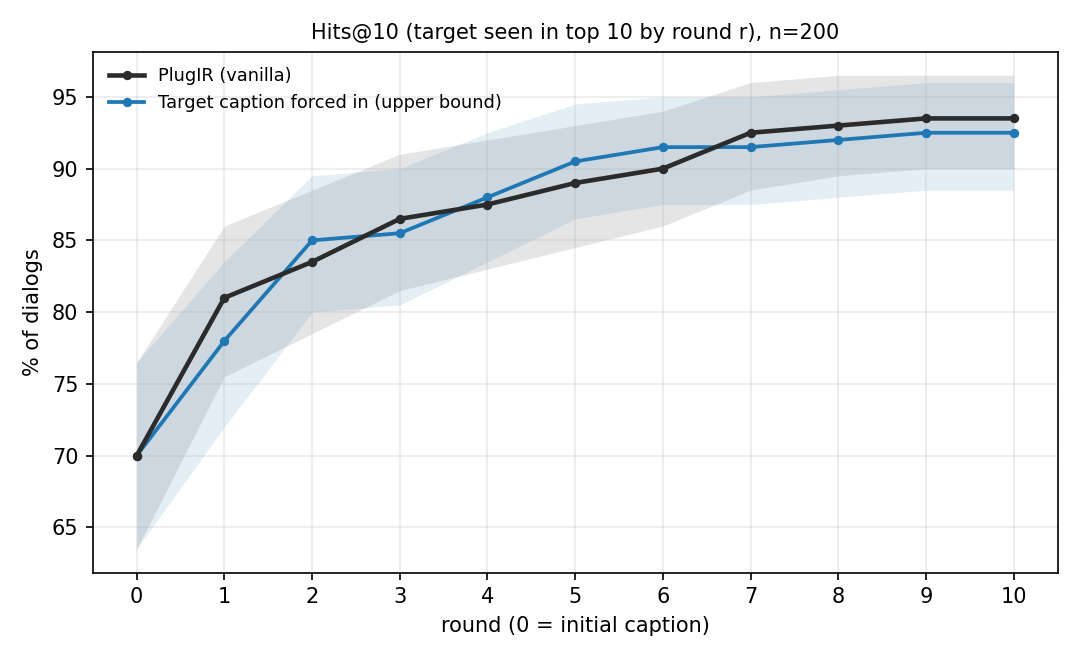
\includegraphics[width=\linewidth]{hits10_curves.png}
\caption{Cumulative Hits@10 by round for vanilla PlugIR and the target-caption upper bound
(200 dialogs, shaded: 95\% bootstrap bands). \runningtodo{replace with the figure that also has
the history-pool and fixed-pool runs (\texttt{runs/v3\_curves/hits10\_curves.png})}}
\label{fig:hits}
\Description{Two nearly overlapping rising curves from 70\% at round 0 to about 93\% at round 10.}
\end{figure}

\paragraph{What we learned.}
\emph{(i) Hits@10 leaves little room.} Vanilla PlugIR already has 70\% of targets in the top 10
before any question and 93.5\% after ten rounds; only 13 of the 200 dialogs never reach the top 10.
\emph{(ii) The evidence shown to the questioner is not the bottleneck.} Offline, better evidence
looks valuable, yet no evidence change moves end-to-end Hits@10 by more than 1.5 points, and
showing the questioner the target's own caption every round does not help at all.
\emph{(iii) Targets are lost after they are found.} 8.5\% of dialogs drop out of the top 10 again,
27\% of rewrites lower the target's rank, and the one query change we tested end to end (S1
fusion) cost 5.5 points.
Together these point away from better question \emph{evidence} and towards how answers become
queries: keeping the best query state, checking a rewrite before committing to it, and using the
agent's own probes for that check, which is the core of our proposal.
\runningtodo{revisit (ii) once the history-pool vs.\ matched-baseline runs finish.}

\paragraph{What we will test next.}
\begin{itemize}
\item Finish the pending runs: history pool vs.\ matched top-100 baseline, fixed top-500 pool and
  best-ranked representatives.
\item \textbf{Query drift}: keep the best query seen so far, or fuse it with the new rewrite, aimed
  at the 8.5\% of dialogs that lose the target.
\item \textbf{Agentic probes}: run the answer-simulation ranker end to end, then let the agent
  issue probes to verify a rewrite and to surface the target directly.
\item \textbf{Harder evaluation}: report Hits@1 and late-round Recall@10 alongside Hits@10, since
  Hits@10 is close to its ceiling.
\end{itemize}

\subsection{Challenges}
\begin{itemize}
\item \textbf{Compute.} With a free 4-bit model on one GPU, each method takes about 4.6 hours for
  200 dialogs (about 18 LLM calls per round), and Colab sessions end when the laptop sleeps. Runs
  resume from saved state; a hosted API for the same model would cut run time roughly tenfold.
\item \textbf{Offline vs.\ live.} Gains measured on saved dialog states (up to 11 points of
  Recall@10) have not survived in new dialogs, so every claim now needs an end-to-end run.
\item \textbf{Model substitution.} Using Qwen3.5-9B instead of ChatGPT and BLIP-2 means our
  absolute numbers are not directly comparable to PlugIR's; we compare variants only within one
  setup.
\end{itemize}

%====================================================================
\section{Team contributions}
\label{sec:team}
\begin{itemize}
\item \textbf{Usman Ali} (ua49): the \textsc{AgentIR} framework (agent modules, simulated user,
  orchestrator, evaluator and tests); the full-dialog diagnostic experiments E1--E3; the
  200-dialog end-to-end runs of the target-caption upper bound and history pooling, and the
  cluster diagnostics.
\item \textbf{Nophar Shalom} (ns2242): the team repository and the port of the original PlugIR code
  to Qwen and Colab; PlugIR dialog visualizations and the saved-state re-analysis.
\item \textbf{Kenechukwu Okoroafor} (kao92): the saved-state experiments on query fusion (S1),
  candidate pools (S2) and caption selectors (S3), and their end-to-end re-runs with Hits@10.
\end{itemize}

\section*{Code}
Repository:\\
\href{https://github.com/nopharshalom/ChatIR-Cornell2026}{\texttt{github.com/nopharshalom/ChatIR-Cornell2026}}\\
The README explains installation and how to run each experiment; the notebook
\texttt{experiments/AgentIR\_v3\_200dialogs.ipynb} reproduces Table~\ref{tab:live}.

\bibliographystyle{ACM-Reference-Format}
\bibliography{refs}

\end{document}
